\section{椭圆中常见的二级结论}

\subsection{焦点三角形面积公式}

\begin{theorem}
    焦点三角形面积公式：如图，设 $P$ 是椭圆 $\frac{x^2}{a^2}+\frac{y^2}{b^2}=1(a>b>0)$ 上一点，$F_1(-c, 0), F_2(c, 0)$分别是椭圆的左、右焦点，$\angle F_1 P F_2=\theta$ ，则 $S_{\triangle P F_1 F_2}=c\left|y_P\right|=b^2 \tan \frac{\theta}{2}$.

    \begin{center}
        \begin{tikzpicture}[scale=0.8]
            \draw[->, thick] (-4,0) -- (4,0) node[below] {$x$};
            \draw[->, thick] (0,-2.5) -- (0,2.5) node[left] {$y$};

            \def\a{3}
            \def\b{2}
            \pgfmathsetmacro{\c}{sqrt(\a*\a - \b*\b)}

            \draw[blue, thick] (0,0) ellipse (\a cm and \b cm);

            \coordinate (F1) at (-\c,0);
            \coordinate (F2) at (\c,0);
            \fill[red] (F1) circle (2pt) node[below] {$F_1$};
            \fill[red] (F2) circle (2pt) node[below] {$F_2$};

            \coordinate (P) at ({1.5*\a*cos(75)},{1.5*\b*sin(37)});
            \draw[purple, thick] (P) -- (F1) node[midway, above left] {$m=|PF_1|$};
            \draw[purple, thick] (P) -- (F2) node[midway, above right] {$n=|PF_2|$};
            % Add angle marking for theta
            \pic [draw, ->, "$\theta$", angle eccentricity=1.5, angle radius=0.3cm] {angle=F1--P--F2};

            \fill[blue] (P) circle (2pt) node[above right] {$P(x_0,y_0)$};
            \node[below left] at (0,0) {$O$};
        \end{tikzpicture}
    \end{center}
    证明过程用到了余弦定理和三角函数的半角公式。
\end{theorem}

\begin{proof}
    第一个焦点三角形面积公式与顶点的纵坐标关系比较大。

    $\triangle P F_1 F_2$ 的边 $F_1 F_2$ 上的高 $h=\left|y_P\right|$ ，所以
    $$
        S_{\triangle P F_1 F_2}=\frac{1}{2}\left|F_1 F_2\right| \cdot h=c\left|y_P\right|
    $$
    第二部分，记 $\left|P F_1\right|=m,\left|P F_2\right|=n$ ，则由椭圆定义，$m+n=2 a$（1）
    $$
        \left|F_1 F_2\right|^2=\left|P F_1\right|^2+\left|P F_2\right|^2-2\left|P F_1\right| \cdot\left|P F_2\right| \cdot \cos \angle F_1 P F_2
    $$
    $$
        4 c^2=m^2+n^2-2 m n \cos \theta=(m+n)^2-2 m n-2 m n \cos \theta
    $$
    将式（1）代入可得：
    $$
        4 c^2=4 a^2-2 m n(1+\cos \theta)
    $$
    $$
        m n=\frac{4 a^2-4 c^2}{2(1+\cos \theta)}=\frac{2 b^2}{1+\cos \theta}
    $$
    $$
        S_{\triangle P F_1 F_2}=\frac{1}{2} m n \sin \theta=\frac{1}{2} \cdot \frac{2 b^2}{1+\cos \theta} \cdot \sin \theta=b^2 \cdot \frac{\sin \theta}{1+\cos \theta}=b^2 \cdot \frac{2 \sin \frac{\theta}{2} \cos \frac{\theta}{2}}{2 \cos ^2 \frac{\theta}{2}}=b^2 \tan \frac{\theta}{2}
    $$
\end{proof}

\begin{problem}
设椭圆 $\frac{x^2}{5}+y^2=1$ 的左、右焦点分别为 $F_1, F_2$ ，点 $M$ 在椭圆 $C$ 上，且 $\angle F_1 M F_2=120^{\circ}$，则 $|O M|=$
\end{problem}

\begin{tips}
    这里 $O$ 为原点。焦点三角形两个面积公式同时考察的题，是 2023 年全国甲卷压轴选择的原型。
\end{tips}

\v{12em}

\begin{problem}
（2023年全国甲卷）
椭圆 $\frac{x^2}{9}+\frac{y^2}{6}=1$ 的两焦点为 $F_1, F_2, O$ 为原点，$P$ 为椭圆上一点， $\cos \angle F_1 P F_2=\frac{3}{5}$ ，则 $|O P|=(\hspace{2em})$
\begin{tasks}(4)
    \task $\frac{2}{5}$
    \task $\frac{\sqrt{30}}{2}$
    \task $\frac{3}{5}$
    \task $\frac{\sqrt{35}}{2}$
\end{tasks}
\end{problem}

\v{12em}

\begin{example}
    （2003 北京卷 15 题）如图，$\mathrm{F}_1, \mathrm{~F}_2$ 分别为椭圆 $\frac{x^2}{a^2}+\frac{y^2}{b^2}=1$ 的左、右焦点，点 P 在椭圆上，$\triangle \mathrm{POF}_2$ 是面积为 $\sqrt{3}$的正三角形，则 $\mathrm{b}^2$ 的值是 \underline{$\qquad$} ．
\end{example}

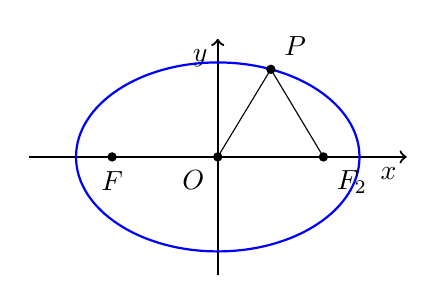
\begin{tikzpicture}[
        scale=0.6,
        point/.style={circle, fill=black, inner sep=1.2pt}
    ]

    \def\a{3}
    \def\b{2}
    \pgfmathsetmacro{\c}{sqrt(\a*\a - \b*\b)}

    \draw[->, thick] (-4,0) -- (4,0) node[below left] {$x$};
    \draw[->, thick] (0,-2.5) -- (0,2.5) node[below left] {$y$};

    \draw[blue, thick] (0,0) ellipse (\a cm and \b cm);

    \coordinate (O) at (0,0);
    \coordinate (F1) at (-\c,0);
    \coordinate (F2) at (\c,0);
    \coordinate (P) at (68:\a cm and \b cm);

    \node[point, label=below left:{$O$}] at (O) {};
    \node[point, label=below:{$F$}] at (F1) {};
    \node[point, label=below right:{$F_2$}] at (F2) {};
    \node[point, label=above right:{$P$}] at (P) {};

    \draw (P) -- (O);
    \draw (P) -- (F2);
\end{tikzpicture}

\v{12em}


\subsection{椭圆的第二定义与焦半径公式}

\begin{definition}[椭圆的准线]
    椭圆的准线是平面内一条与椭圆焦点 $F$ 距离成比例的直线，准线方程为 $x = \pm \frac{a^2}{c}$（焦点在 $x$ 轴上）或 $y = \pm \frac{a^2}{c}$（焦点在 $y$ 轴上），其中 $c$ 是椭圆的焦距。

    \begin{center}
        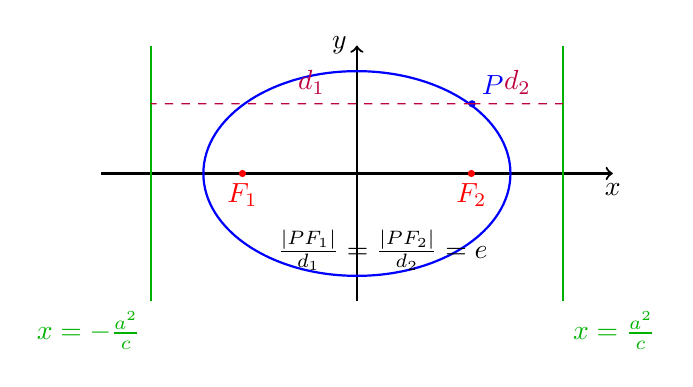
\begin{tikzpicture}[scale=0.65]
            \draw[->, thick] (-5,0) -- (5,0) node[below] {$x$};
            \draw[->, thick] (0,-2.5) -- (0,2.5) node[left] {$y$};

            \def\a{3}
            \def\b{2}
            \pgfmathsetmacro{\c}{sqrt(\a*\a - \b*\b)}
            \pgfmathsetmacro{\d}{\a*\a/\c}

            \draw[blue, thick] (0,0) ellipse (\a cm and \b cm);

            \coordinate (F1) at (-\c,0);
            \coordinate (F2) at (\c,0);
            \fill[red] (F1) circle (2pt) node[below] {$F_1$};
            \fill[red] (F2) circle (2pt) node[below] {$F_2$};

            \coordinate (P) at ({1.5*\a*cos(60)},{1.5*\b*sin(27)});
            \fill[blue] (P) circle (2pt) node[above right] {$P$};

            \draw[green!70!black, thick] (\d,2.5) -- (\d,-2.5) node[below right] {$x=\frac{a^2}{c}$};
            \draw[green!70!black, thick] (-\d,2.5) -- (-\d,-2.5) node[below left] {$x=-\frac{a^2}{c}$};

            \draw[purple, dashed] (P) -- ({\d},{1.5*\b*sin(27)}) node[midway, above] {$d_2$};
            \draw[purple, dashed] (P) -- ({-\d},{1.5*\b*sin(27)}) node[midway, above] {$d_1$};

            \node at (0.5,-1.5) {$\frac{|PF_1|}{d_1} = \frac{|PF_2|}{d_2} = e$};
        \end{tikzpicture}
    \end{center}
\end{definition}

\begin{definition}[第二定义]
    \textbf{椭圆}是平面内一动点到定点与到准线的距离比是常数的点的轨迹 $e = \frac{|PF_i|}{d_i}$（其中 $i = 1,2$）。
    \begin{tips}
        用的很少，除非冲 140+，否则不用管。
    \end{tips}
\end{definition}

\begin{example}
    已知动点 $P(x, y)$ 满足 $10 \sqrt{(x-1)^2+(y-2)^2}=|3 \mathrm{x}+4 \mathrm{y}+2|$ ，则动点 P 的轨迹是 （\qquad）
    \begin{tasks}(4)
        \task 椭圆
        \task 双曲线
        \task 抛物线
        \task 无法确定
    \end{tasks}
\end{example}

\v{4em}

\begin{example}
    椭圆 $\frac{x^2}{25}+\frac{y^2}{16}=1$ 外一点 $A(5,6)$,椭圆上一点 $P$，$l$ 为椭圆的左准线，点 $P$ 到 $l$ 的距离为 $d$ ，则 $P A+\frac{3}{5} d$ 的最小值为
\end{example}

\v{10em}

\begin{definition}[椭圆的焦半径公式]
    椭圆上任意一点 $P$ 到焦点 $F$ 的距离称为焦半径，记作 $|PF|$。对于椭圆 $\frac{x^2}{a^2} + \frac{y^2}{b^2} = 1 (a > b > 0)$，根据椭圆第二定义有：
    $$
        \begin{aligned}
             & \left|P F_1\right|=e\left(x_0+\frac{a^2}{c}\right)=a+e x_0 \\
             & \left|P F_2\right|=e\left(\frac{a^2}{c}-x_0\right)=a-e x_0
        \end{aligned}
    $$
    此为椭圆的焦半径公式。
    \begin{center}
        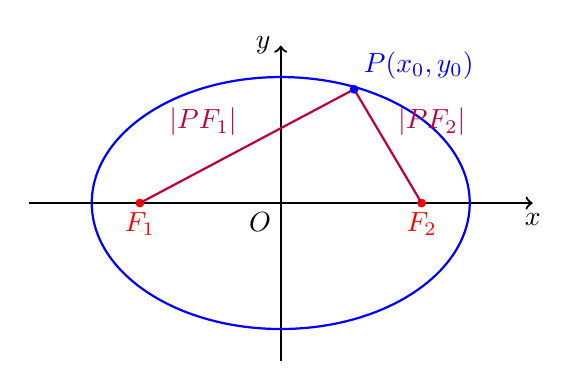
\begin{tikzpicture}[scale=0.8]
            \draw[->, thick] (-4,0) -- (4,0) node[below] {$x$};
            \draw[->, thick] (0,-2.5) -- (0,2.5) node[left] {$y$};

            \def\a{3}
            \def\b{2}
            \pgfmathsetmacro{\c}{sqrt(\a*\a - \b*\b)}

            \draw[blue, thick] (0,0) ellipse (\a cm and \b cm);

            \coordinate (F1) at (-\c,0);
            \coordinate (F2) at (\c,0);
            \fill[red] (F1) circle (2pt) node[below] {$F_1$};
            \fill[red] (F2) circle (2pt) node[below] {$F_2$};

            \coordinate (P) at ({1.5*\a*cos(75)},{1.5*\b*sin(37)});
            \draw[purple, thick] (P) -- (F1) node[midway, above left] {$|PF_1|$};
            \draw[purple, thick] (P) -- (F2) node[midway, above right] {$|PF_2|$};

            \fill[blue] (P) circle (2pt) node[above right] {$P(x_0,y_0)$};
            \node[below left] at (0,0) {$O$};
        \end{tikzpicture}
    \end{center}
\end{definition}

\begin{example}
    椭圆 $\frac{x^2}{25}+\frac{y^2}{16}=1$ 上的点 $M$ 到左准线的距离是 2.5 ，则 $M$ 到左焦点的距离为 \underline{\qquad} ，$M$ 到右焦点的距离为 \underline{\qquad}
\end{example}

\v{4em}

\begin{example}
    已知 $A, ~ B$ 为椭圆 $\frac{x^2}{9}+\frac{y^2}{5}=1$ 上两个不同的点，$F$ 为右焦点，$|A F|+|B F|=4$ ，若线段 $A B$ 的垂直平分线交 $x$ 轴于点 $T$ ，则 $|F T|=$ \underline{\qquad}.
\end{example}

\begin{tips}
    利用焦半径公式和点差法构造
\end{tips}

\begin{solution}
    \begin{minipage}[c]{0.55\textwidth}
        由焦半径公式：$\left(3-\frac{2}{3} x_1\right)+\left(3-\frac{2}{3} x_2\right)=4$ 得：$x_1+x_2=3$

        即 $A B$ 中点 $\left(\frac{3}{2}, \frac{y_1+y_2}{2}\right), T(m, 0), ~ k_{A B}=\frac{y_1-y_2}{x_1-x_2}$

        则 $A B$ 垂直平分线斜率为 $-\frac{x_1-x_2}{y_1-y_2}$

        根据点 $A, B$ 在椭圆上，则有 $\frac{x_1^2}{9}+\frac{y_1^2}{5}=1, ~ \frac{x_2^2}{9}+\frac{y_2^2}{5}=1$

        作差化简得 $y_1^2-y_2^2=\frac{5}{9}\left(x_2^2-x_1^2\right)$

        则线段 $A B$ 的垂直平分线方程为 $y=-\frac{x_1-x_2}{y_1-y_2}\left(x-\frac{3}{2}\right)+\frac{y_1+y_2}{2}$

        代入 $T(m, 0)$ 得： $m-\frac{3}{2}=\frac{y_1^2-y_2^2}{2\left(x_1-x_2\right)}=\frac{\frac{5}{9}\left(x_2^2-x_1^2\right)}{2\left(x_1-x_2\right)}=-\frac{\frac{5}{9}\left(x_1+x_2\right)}{2}=-\frac{5}{6}$

        即 $x_0=\frac{2}{3}$ ，则 $|F T|=2-\frac{2}{3}=\frac{4}{3}$ ．故答案为：$\frac{4}{3}$ ．
    \end{minipage} %
    \begin{minipage}[c]{0.4\textwidth}
        \begin{figure} [H]
            \centering
            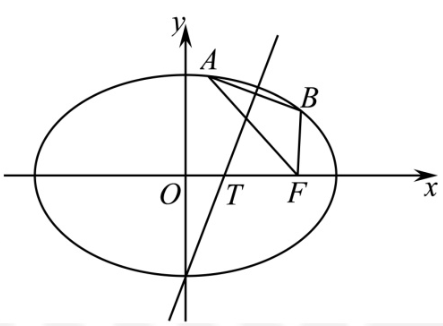
\includegraphics[width=0.6\textwidth]{chapters/圆锥曲线/images/椭圆/img-20250730180354.png}
        \end{figure}
    \end{minipage}
\end{solution}

\subsection{第三定义}

\begin{definition}
    平面内的动点到两定点 $A_1\left(a_1, 0\right)$、$A_2\left(a_2, 0\right)$（或 $A_1\left(0, a_1\right) A_2\left(0, a_2\right)$ ）的斜率乘积等于常数 $e^2-1$ 的点的轨迹叫做椭圆或双曲线，其中两定点分别为椭圆或双曲线的顶点；
\end{definition}

\begin{theorem}
    当常数大于 -1 小于 0 时为椭圆，当常数大于 0 时为双曲线。

    由第三定义知：$A$、$B$ 为椭圆或双曲线的顶点，$P$ 是椭圆上异于 $A$、$B$ 的一点，若 $k_{P A}$、$k_{P B}$ 存在，

    则有：$k_{P A} \cdot k_{P B}=e^2-1$ ．
\end{theorem}

\begin{example}
    $P$ 是双曲线 ：$\frac{x^2}{a^2}-\frac{y^2}{b^2}=1$，$(a>0, b>0)$ 上一点，$M, ~ N$ 分别是双曲线的左右顶点，直线 $P M, ~ P N$ 的斜率之积为 $\frac{1}{5}$ ，则双曲线离心率为（\hspace{2em}）。
\end{example}

\begin{example}
    已知 $A$、$B$ 是椭圆 $\frac{x^2}{a^2}+\frac{y^2}{b^2}=1(a>b>0)$ 长轴的两个端点，$M$、$N$ 是椭圆上关于 $x$ 轴对称的两点，直线 $A M$、$B N$ 的斜率分别为 $k_1$、$k_2$ ，且 $k_1 k_2 \neq 0$ 若 $\left|k_1\right|+\left|k_2\right|$ 的最小值为 1 ，则椭圆的离心率为（\hspace{2em}）

    \begin{figure} [H]
        \centering
        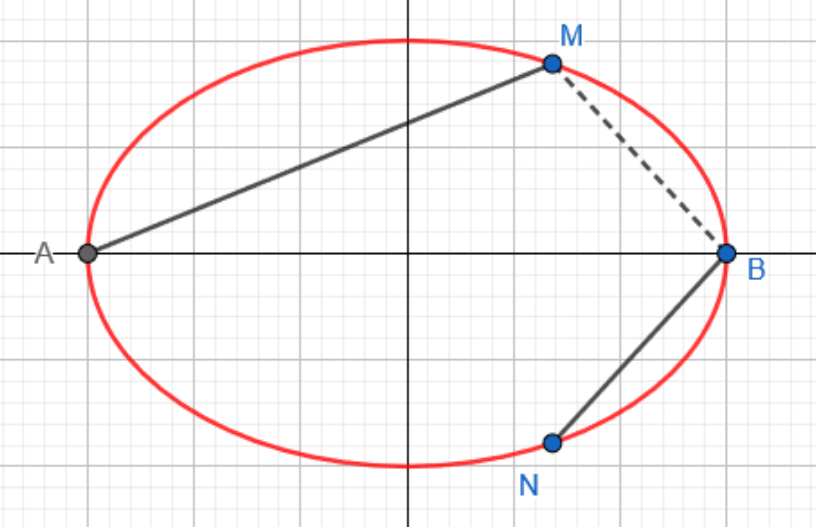
\includegraphics[width=0.3\textwidth]{chapters/圆锥曲线/images/椭圆中常见的二级结论/img-20250602104154.png}
    \end{figure}

\end{example}


\begin{solution}
    连接 $M B$ ，由椭圆的第三定义可知：$k_{A M} \cdot k_{B M}=e^2-1=-\frac{b^2}{a^2}$ ，而 $k_{B M}=-k_{B N}$ ，所以 $k_1 k_2=\frac{b^2}{a^2}$ ，

    $$
        \left|k_1\right|+\left|k_2\right| \geq 2 \sqrt{\left|k_1\right| \cdot\left|k_2\right|}=\frac{2 b}{a}=1
    $$

    因此 $e=\frac{\sqrt{3}}{2}$.

    \begin{note}
        在椭圆中，$ e^2-1 = - \frac{b^2}{a^2}$，双曲线中是$ e^2-1 = + \frac{b^2}{a^2}$，代进去就知道了。
    \end{note}
\end{solution}

\vspace{2em}

\begin{problem}
已知点 $A(-5,0), B(5,0)$ ，动点 $P(m, n)$ 满足直线 $P A, P B$ 的斜率之积为 $-\frac{16}{25}$ ，则 $4 m^2+n^2$ 的取值范围是
\begin{tasks}(4)
    \task $[16,100]$
    \task $[25,100]$
    \task $[16,100)$
    \task $(25,100)$
\end{tasks}
\end{problem}

\subsection{中点弦}

\begin{definition}
    弦取了一个中点，也会满足斜率之积为 $e^2-1$。下图展现了所有可能出现的情况：

    \begin{figure} [H]
        \centering
        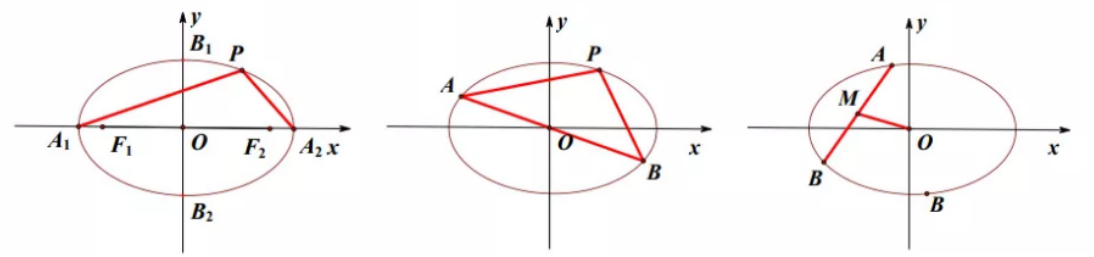
\includegraphics[width=0.7\textwidth]{chapters/圆锥曲线/images/椭圆中常见的二级结论/img-20250602105059.png}
    \end{figure}
\end{definition}

\begin{definition}
    在双曲线里也会有的：

    \begin{figure} [H]
        \centering
        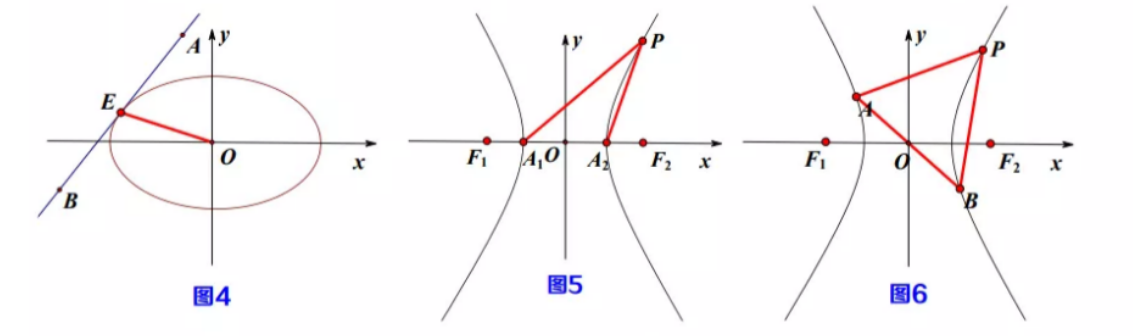
\includegraphics[width=0.65\textwidth]{chapters/圆锥曲线/images/椭圆中常见的二级结论/img-20250602105130.png}
    \end{figure}

\end{definition}

\begin{example}
    过 $M(2,1)$ 作$k=-1$ 的直线与椭圆 $C: \frac{x^2}{a^2}+\frac{y^2}{b^2}=1$ 相交于 $A, B$ 两点，若 $M$ 为线段 $A B$ 的中点，则 $C$ 的离心率为
    \begin{tasks}(4)
        \task $\frac{1}{3}$
        \task $\frac{\sqrt{2}}{3}$
        \task $\frac{1}{2}$
        \task $\frac{\sqrt{2}}{2}$
    \end{tasks}
\end{example}

\v{8em}

\begin{example}
    直线 $3 x+4 y-11=0$ 与椭圆 $\frac{x^2}{4}+\frac{y^2}{m^2}=1$ 交于 $A, B$ 两点，若点 $P(1,2)$ 恰为弦 $A B$ 的中点，则椭圆的离心率是
    \begin{tasks}(4)
        \task $\frac{\sqrt{3}}{3}$
        \task $\frac{\sqrt{2}}{2}$
        \task $\frac{\sqrt{3}}{2}$
        \task $\frac{\sqrt{6}}{3}$
    \end{tasks}
\end{example}

\v{8em}

\begin{example}
    已知直线 $x+y-1=0$ 与椭圆 $C: b^2 x^2+a^2 y^2=a^2 b^2(a>b>0)$ 相交于 $A, B$ 两点，且线段 $A B$ 的中点 $M$ 在直线 $l: x-2 y=0$ 上，则椭圆 $C$ 的离心率为
    \begin{tasks}(4)
        \task $\frac{\sqrt{2}}{2}$
        \task $\frac{\sqrt{3}}{2}$
        \task $\sqrt{2}$
        \task $\frac{1}{2}$
    \end{tasks}
\end{example}

\v{8em}

\begin{example}
    椭圆的 $F$ 为左焦点，$P$ 为下顶点，平行于 $F P$ 的直线交椭圆于 $A, B$ 两点，且 $A B$ 的中点为 $M\left(1, \frac{1}{2}\right)$ ，则椭圆离心率为
    \begin{tasks}(4)
        \task $\frac{\sqrt{2}}{2}$
        \task $\frac{1}{2}$
        \task $\frac{1}{4}$
        \task $\frac{\sqrt{3}}{2}$
    \end{tasks}
\end{example}

\v{8em}